% Template for ICASSP-2020 paper; to be used with:
%          spconf.sty  - ICASSP/ICIP LaTeX style file, and
%          IEEEbib.bst - IEEE bibliography style file.
% --------------------------------------------------------------------------
\documentclass{article}
\usepackage{spconf,amsmath,graphicx}
\usepackage{color,soul}
\usepackage{algorithm2e}

% Example definitions.
% --------------------
\def\x{{\mathbf x}}
\def\L{{\cal L}}

% Title.
% ------
\title{Extracting Hip-Hop Instrumental Music\\By Exploiting Repeating Structure}
%
% Single address.
% ---------------
\name{Cole Peterson, George Tzanetakis}
\address{University of Victoria\\\texttt{cpeterso@uvic.ca}, \texttt{gtzan@uvic.ca}}
%
% For example:
% ------------
%\address{School\\
%	Department\\
%	Address}
%
% Two addresses (uncomment and modify for two-address case).
% ----------------------------------------------------------
%\twoauthors
%  {A. Author-one, B. Author-two\sthanks{Thanks to XYZ agency for funding.}}
%	{School A-B\\
%	Department A-B\\
%	Address A-B}
%  {C. Author-three, D. Author-four\sthanks{The fourth author performed the work
%	while at ...}}
%	{School C-D\\
%	Department C-D\\
%	Address C-D}
%
\begin{document}
%\ninept
%
\maketitle
%
\begin{abstract}
Many source separation algorithms take advantage of repeating musical structures to better separate the voice from accompanying instrumental music. Hip-hop music is especially repetitive, often using identical loops under non-repeating rap lyrics. In this paper, we present a method for separating instrumental music and vocals in hip-hop by first identifying similar sound segments in the track's magnitude spectrogram, and then reconstructing an estimate of those repeating sounds. Our approach is based on the repeating pattern extraction technique (REPET) with modifications that improve its performance for hip-hop music; we modify it by finding optimal segment alignment and using a minimum operator in place of a medium operator. We evaluate performance on a newly-assembled dataset of 50 popular hip-hop tracks and their instrumentals, as well as an existing dataset of 100 tracks containing a wider variety of music.
Our experiments show that the proposed method can effectively separate full hip-hop tracks better than existing approaches, but this improvement is limited to hip-hop and other music with strong repeating structure. 
\end{abstract}
%
\begin{keywords}
Sound source separation, instrumental extraction, REPET
\end{keywords}
%
\section{Introduction}\label{sec:introduction}

%Hip-hop culture values its instrumentals more than other genres do. 
Hip-hop instrumentals have many uses, and this creates a demand for them. Instrumentals are reused by different rappers to release ``mix-tapes'', collections of songs less polished and less original than would be released on a proper album, they are used in battle rap competitions and by freestylers (rappers who improvise lyrics over a beat), they are used by remixers to blend two existing rap songs by putting the rap verse of one over the instrumental beat of another, and they are used by amateurs to perform karaoke. The demand for these instrumentals and the sampling culture of hip-hop means that many instrumentals are given an official release, so ground truth is easier to come by for evaluating automated sound source separation. A new dataset of 50 songs, from varying artists and time periods, was created to evaluate the separation of hip-hop music, and guide the design and development of our algorithm. 

The repetitive nature of hip-hop instrumentals (often composed of identical loops) also lends itself to sound source separation techniques that leverage repetition. The original REPET algorithm\cite{REPET} models music as a repeating background and non-repeating foreground, using repeating features of the sound to separate it. REPET segments the magnitude spectrogram into equally sized pieces, and then derives a ``repeating mask'' a soft-mask which estimates the repeating sounds in each segment and is used to filter every segment in the input sound. This method works well for short segments of music where the musical structure remains static, however it struggles to effectively separate full songs as it does not adapt over time to changes in the music. Several adaptations of the ideas in the original REPET algorithm have been produced to handle this common ``verse-chorus'' problem. Both repet\_ada \cite{filtering}, and repet\_seg \cite{REPET} look for repeating patterns locally, however, they do not take advantage of similar sounds which may appear far away from each other (e.g. instrumentals in the 1st verse and 3rd verse), nor does it exclude dissimilar sounds which appear close to each other (e.g. a verse right next to a chorus). 

Adaptive REPET (repet\_ada)\cite{filtering} keeps track of a beat spectrogram, representing how the repeating period changes over the course of a song. It uses this beat spectrogram to find the repeating period $p$ for each time slice, and then calculates the element-wise median of the two time slices $\pm p$ away from it for use in the repeating mask. Segmented REPET (repet\_seg)\cite{REPET} performs the original REPET algorithm on overlapping windows of a set size (with 10s shown to be optimal in \cite{REPET}), overcoming original REPET's difficulty scaling to long songs by dividing it into smaller sounds. Both of these approaches are highly local, in repet\_ada the repeating mask is determined by sounds $p$ away, and in repet\_seg the window size limits where repeating sounds can be found.

Like those adaptations, this paper presents a method that uses a \emph{dynamic} repeating mask, which is able to change over the course of the song. The repeating mask is calculated by selecting a set number of segments of sound from anywhere in the track which are expected to contain the same or similar backgrounds. Additionally, while REPET and its variants use an element-wise median on the segments of the magnitude spectrogram, this paper suggests better results can be obtained by taking the minimum of the selected segments as a frequency mask. 

\section{Related Work} 


Audio source separation has been a topic of active research for
several years. The Signal Separation Evaluation Compaign (SiSEC) has
been instrumental in providing data sets and tasks for evaluating
different algorithms \cite{sisec, Vincent:2012ab,stoter20182018}. A large variety of
algorithms have been proposed for this task \cite{bayes,
  Haddad:2008aa}. In the most general setting no assumptions are made
about the different sound sources in the mixture. A large number of
work in audio source separation focuses on speech signal
\cite{DNNSpeech, DNNSpech2} but more recently music signals have also
been analyzed. Music provides a particularly interesting case as some
sound sources can be considered more important than others (for
example vocals) and assumptions about structure and repetition 
can be used to improve the separation performance \cite{Dannenberg:2008aa}. 
The term informed sound source separation has been used to describe 
such algorithms \cite{liutkus:hal-00958661}. Deep recurrent neural networks have been
explored for signing voice separation \cite{DNNSing}. Other approaches
are based on non-negative matrix factorization \cite{fasst} or utilize
pitch and rhythmic information \cite{Rafii:2014aa}. Our proposed
approach belongs to a family of methods that leverage the strong
repetition in musical signals that originate from the REPET (REpeating
Pattern Extraction Technique) method \cite{separation, REPET, online,
  filtering}. There are several approaches that have been proposed to
evaluate the performance of blind and informed sound source separation
algorithms \cite{Vincent:2006aa, emiya:inria-00567152} originating
from the audio source separation evaluation campaigns \cite{BSS,
  Vincent:2012ab}.

\section{Method}

Early stages of the algorithm match the REPET algorithm described in \cite{separation}. A spectrogram of the input signal, $X$, is calculated using a Short-Time Fourier Transform with a Hamming window and constant overlap. The magnitude spectrogram, $V$, is derived from $X$ without the mirrored frequencies. The repeating period, $p$, is determined from autocorrelating each frequency bin of $V^2$, and taking the mean of the results. 

\begin{figure}[h]
	\caption{Outline of the xcorr\_min REPET algorithm}
	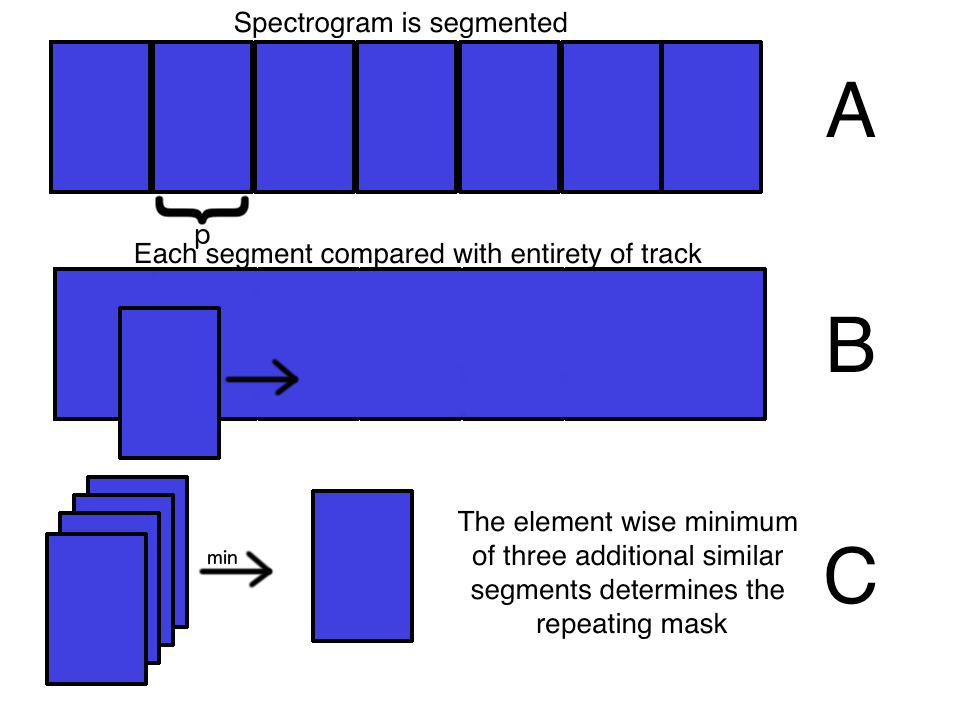
\includegraphics[width=0.5\textwidth]{figs/xcorr_min.png}
	\label{fig:REPET}
\end{figure}

\subsection{Similar Segment Identification}

A visual outline of the salient part of this algorithm can been seen in Figure \ref{fig:REPET}. Like in the original REPET the magnitude spectrogram $V$ is divided into segments of size $p$ (step A in Figure \ref{fig:REPET}), however we then compare each of these segments to every alignment possible over entirety of $V$(step B Figure \ref{fig:REPET}). This allows us to find multiple similar sounding segments from anywhere in the track, while standard REPET uses its neighbouring segments (those which are offset by a multiple of $p$). Within local ranges the most similar segments of sound are often found offset by $p$, but can become misaligned over longer durations. We find better segments when not constraining the segments to a multiple of the repeating period: we search for the optimal alignment, using $p$ only to determine the size of the segments. This provides for better results, but does come at a high computational cost, making this method slower than existing REPET methods.  Given a $p$-length segment $S$, we identify 3 similar sounding segments by the process shown in Algorithm 1, which is essentially choosing the maximum 3 segments of a modified cross correlation between $S$ and $V$.

\begin{algorithm}
	\KwData{Magnitude Spectrogram $V$, Segment Magnitude Spectrogram $S$}
	\KwResult{3 similar sounding segments for each segment}
		$\vert s \vert = length(S)$;\\
		$\vert v \vert = length(V)$;\\
		\For{i in ($\vert v \vert - \vert s \vert$)} { 
			similarity[i] = dot($S$,min($S$,V[i:i+p]));\\
			//dot(A,B) is the inner product of A and B
		}
		\For{3 iterations} {
			j = argmax(similarity);\\
			add V[j:j+p] to similar segments of segment $S$;\\
			remove indexes in the range $j \pm /2$ from similarity;\\
		}
	\caption{Identification of 3 similar segments}
\end{algorithm}

%We compute a \emph{dynamic repeating mask} for each $p$-length segment $S$ which is unique for every segment and is determined by selecting 3 segments of sound within $V$ which ideally contain the same underlying instrumental music as $S$. These segments can come from anywhere within $V$. We select 3 different segments of similar sound within $V$ using a modified cross-correlation.  The similarity at every point in $V$ is calculated by taking the dot product between $S$ and the element-wise minimum of $S$ and $V$ from $i$ to $i+p$. Taking the element-wise minimum before the dot product helps prevent selecting segments which will over restrict the repeating mask filter, as it limits the amount an element in $V_{i:i+p}$ can boost the similarity to the amount that exists in $S$.  In other words, taking the dot product with the element-wise minimum minimizes how much sound a segment will filter out, as the operation on the segments is an element-wise minimum. 



%I regret not trying a cosine similarity here -- I realize that this might have done better than this modified dot product, and would have been more elegant. 

\subsection{Segment Operation}
Once we have three similar sounding segments to our original segment, we compute a repeating mask, a soft mask used to filter the input signal. This repeating mask is entirely dynamic and will change for every segment, because each segment will have identified different segments which sound similar to it. The challenge then becomes determining the common sounds between the original segment and the three found elsewhere in $V$ which sound similar. Many REPET-like algorithms take an element-wise median for every segment to calculate the repeating mask, although the mean has also been explored. We propose using an element-wise minimum operation (shown in step C of Figure \ref{fig:REPET}) to calculate the repeating mask.



\hl{We justify the use of the minimum operator as follows: If you add a sound $y(t)$ to $x(t)$, you would expect the magnitude spectrogram of the mixture to be greater than that of the original. This is because of the linear property of the Fourier transform,} $\mathcal{F}\{x(t)\} = X(\omega)$ and $\mathcal{F}\{y_n(t)\}  = Y_n(\omega)$: $\mathcal{F}\{x(t)+y_n(t)\}  = X(\omega) + Y_n(\omega)$, so $|X(\omega)+Y(\omega)| > |X(\omega)|$

\hl{If you have multiple copies of x(t), added to different sounds $y_n(t)$, knowing that the original is less than each of the mixtures, you could take the minimum to recover the original sound. }


\begin{equation}\label{Fourier}
\begin{split}
	x(t) \approx \mathcal{F}^{-1} \{min(& |X(\omega) + Y_1(\omega)|, \\
	&|X(\omega) + Y_2(\omega)|, \\
	&|X(\omega) + Y_3(\omega)|, \\
	&|X(\omega) + Y_4(\omega)| )\}
\end{split}
\end{equation}
%This is far from an equality, but my intuition is that in the average case this is pretty close to being true.


\section{Datasets}
Sound source algorithms were evaluated with two datasets:t

\subsection{Hip-hop}
A new dataset of 50 hip-hop tracks spread out over four decades of hip hop was compiled for evaluating and training. Full tracks were used wherever possible, occasionally clipping out ``skit'' intros. All tracks and their instrumentals had a sampling frequency of 44,100Hz, and were comprised of two stereo channels. As most released instrumentals were not properly aligned with their full tracks, this was done by hand in creating the dataset.

\subsection{SiSEC MSD100 Dataset}
The Signal Separation Evaluation Campaign has released the Mixing Secret Dataset, a collection of 100 songs split across genres for setting a benchmark for sound source separation. Following success on a strictly hip-hop dataset, the version of REPET was run on this general music dataset to gauge its performance on music in general. This dataset is also sampled at 44,100Hz, and has source files for drum, bass, vocals, and other. We considered the instrumental to be the combination of bass, drums, and other, and tested our output against that.


\section{Evaluation}


Results were evaluated using Blind Source Separation Evaluation (BSS Eval) \cite{BSS}. This provides four objective measures of sound separation quality between a source and its estimate, a source to distortion ratio (SDR), source image to spatial distortion (ISR), source to interferences ratio (SIR), and source to artifact ratio (SAR). A better separation will yield higher values. Figure \ref{fig:SDR_hip_hop} shows comparative results between REPET algorithms on the hip-hop dataset, Figure \ref{fig:SDR_MSD} shows the result on the MSD100 dataset. Table \ref{tab:percentBest_hip_hop} shows how often each algorithm presents the best results for each of the BSS categories in the hip-hop dataset.

  \begin{table}[h]
  \caption{Number of songs each algorithm gives the best result for each BSS measure on the hip-hop dataset.}
  \label{tab:percentBest_hip_hop}
  \begin{center}
  \begin{tabular}{@{} cccc @{}}
    \hline
    & xcorr\_min & repet\_ada & repet\_seg \\ 
    \hline
    SDR & \textbf{29} & 1 & 20 \\ 
    ISR & \textbf{32} & 6 & 12 \\ 
    SIR & \textbf{19} & 14 & 17 \\ 
    SAR & \textbf{33} & 1 & 16\\
    \hline
  \end{tabular}
      \end{center}
    \end{table}

\begin{figure}[h]
	\caption{SDR performance of different methods on hip-hop dataset.}
	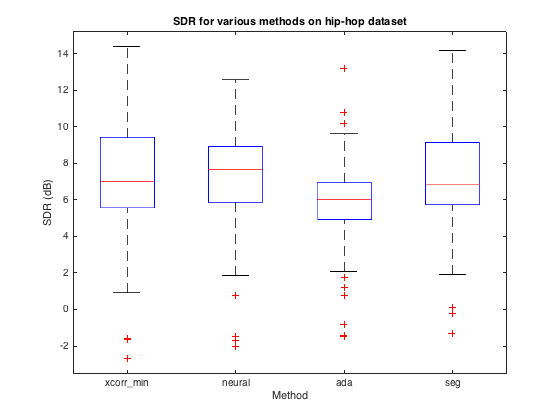
\includegraphics[width=0.5\textwidth]{figs/allSDR_inc_neural_hip_hop_new.png}
	\label{fig:SDR_hip_hop}
\end{figure}

%\begin{figure}[h]
%	\caption{SDR performance of different methods on MSD100 dataset.}
%	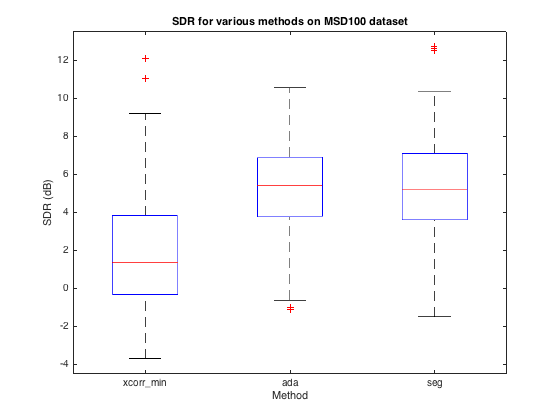
\includegraphics[width=0.5\textwidth]{figs/allSDR_MSD100_new.png}
%	\label{fig:SDR_MSD}
%\end{figure}


  \begin{table}[h]
  \caption{Mean and standard deviation performance for each algorithm on the hip-hop dataset}
  \label{tab:meanHipHop}
  \begin{tabular}{@{} ccccc @{}}
    \hline
  & SDR & ISR & SIR & SAR \\
    \hline
xcorr\_min & 7.1 $\pm$ 3.8 & \textbf{13.8 $\pm$ 5.8} & 23.5 $\pm$ 5.0 & 8.7 $\pm$ 4.3 \\ 
xcorr\_neu & \textbf{7.1 $\pm$ 3.3} & 12.9 $\pm$ 5.0 & 23.8 $\pm$ 4.3 & \textbf{8.8 $\pm$ 4.0} \\ 
repet\_ada & 5.6 $\pm$ 2.9 & 13.1 $\pm$ 5.2 & 26.2 $\pm$ 5.1 & 6.2 $\pm$ 3.5 \\ 
repet\_seg & 6.8 $\pm$ 3.0 & 13.3 $\pm$ 5.3 & \textbf{26.5 $\pm$ 5.1} & 7.7 $\pm$ 3.6 \\ 
    \hline
  \end{tabular}
    \end{table}

  \begin{table}[h]
  \caption{Mean and standard deviation performance for each algorithm on the MSD100 dataset}
  \label{tab:meanMSD}
  \begin{tabular}{@{} ccccc @{}}
    \hline
 & SDR & ISR & SIR & SAR \\
    \hline
xcorr\_min & 1.9 $\pm$ 3.1 & 9.5 $\pm$ 3.8 & 30.2 $\pm$ 35.2 & 5.2 $\pm$ 2.5 \\ 
repet\_ada & 5.2 $\pm$ 2.6 & \textbf{14.6 $\pm$ 3.4} & \textbf{36.5 $\pm$ 32.7} & 7.0 $\pm$ 2.2 \\ 
repet\_seg & \textbf{5.3 $\pm$ 2.9} & 14.1 $\pm$ 4.0 & 36.4 $\pm$ 32.7 & \textbf{7.3 $\pm$ 2.4} \\ 
    \hline
  \end{tabular}
    \end{table}

Results within the hip-hop dataset show that the xcorr\_min version of REPET presented in this paper outperform repet\_ada and repet\_seg at the mean and different percentiles. However, we find that the subjective quality of the instrumentals extracted by xcorr\_min greatly exceed the results in any of the other methods, which is not adequately captured in the bss\_eval numbers. 

%\begin{figure}[h]
%	\caption{SDR performance of different methods hip-hop dataset}
%	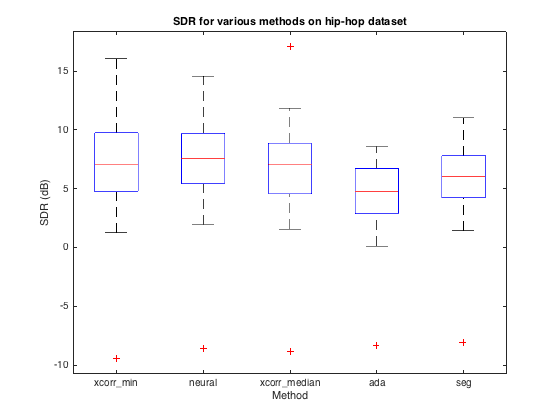
\includegraphics[width=0.5\textwidth]{figs/allSDR_inc_median_hip_hop.png}
%	\label{fig:median}
%\end{figure}

We also tested our optimal alignment approach with an element-wise median (as is used in other REPET approaches) to isolate the effect of that modification to the system. This produced better results than either repet\_ada or repet\_sim, but did not perform as well as xcorr\_min. 

\section{Discussion and future work}\label{sec:limit}




In the process of experimenting with hip-hop tracks we discovered two
limitations of the proposed method: 1) muted end loops, 2) stereo
signals. A common technique in hip-hop production is to mute the
instrumental at the end of a line to place emphasis on the lyrics. In
the data set, this can be seen in ``All Caps'' (all\-caps.wav), and
``Ain't No Half Steppin'" (half.wav), among others. However, if one of
these segments is chosen for use with a segment where the end of the
loop is not muted, this will over restrict the repeating mask, and
only allow the frequencies that are present in the vocal. For example,
consider a loop that repeats four times, and on the fourth, the end is
muted. The algorithm put forward in this paper will use a repeating
mask that eliminates instrumental frequencies at the end of the loop,
when the right choice would be to keep those frequencies in the mask,
as when considering the output for the fourth loop only the
frequencies present in the segment will be output and not those in the
mask (Stage 3 of REPET).

REPET treats the two channels independent of one another, but this
neglects additional and potentially valuable information present in
the other channel. Any sounds that change channels will be thrown
out by the repeating mask. It should also be noted that stereo
features could be used to improve the separation, as vocals are
usually panned in the center, whereas instrumental sounds are often
panned more to the right or left channels. In some cases, subtracting
the one channel from another in the time-domain can result in
surprisingly good separation.

In the future we plan to add automatic detection of muted-end loops
and incorporate stereo panning information in the creation of the mask
to improve vocal separation without making the strong assumption that
vocals are always centered.  We also would plan to do a human evaluation
of the sound source separations, as the perceptual quality of the 
separated vocals and instrumentals is not always
perfectly correlated with the SDR (or other objective metric)
value. This is something that is known in the audio source separation
community and has led to the development of the Perceptual Audio
Source Separation toolkit \cite{peass} which we plan to use. 

From our experiments it is clear that the proposed method performs
better in hip-hop music but not as well in the more general MSD100
data set.  We plan to investigate the automatic detection of which
variant of the algorithm is more appropriate as a way to improve the
results. To support reproducibility the code and associated data set 
described in this paper are available by request from the authors. 



%\nocite{*}
% For bibtex users:
\bibliographystyle{IEEEbib}
\bibliography{b}


\end{document}